\documentclass[11pt,a4paper]{article}

\usepackage{fullpage}
\usepackage[T1]{fontenc}
\usepackage{lmodern}

\usepackage{graphicx}
\usepackage{subcaption}

\begin{document}

\begin{figure}
    \centering
    \begin{subfigure}[b]{0.45\textwidth}
        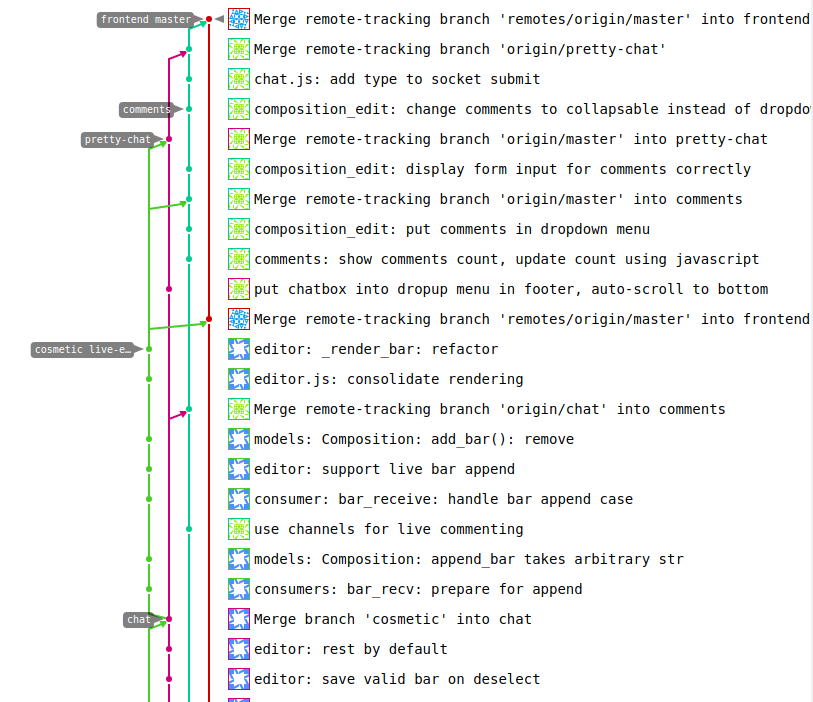
\includegraphics[width=\textwidth]{graph-end-beg}
        \caption{Commits at the beginning and end of an iteration}
    \end{subfigure}
    \begin{subfigure}[b]{0.45\textwidth}
        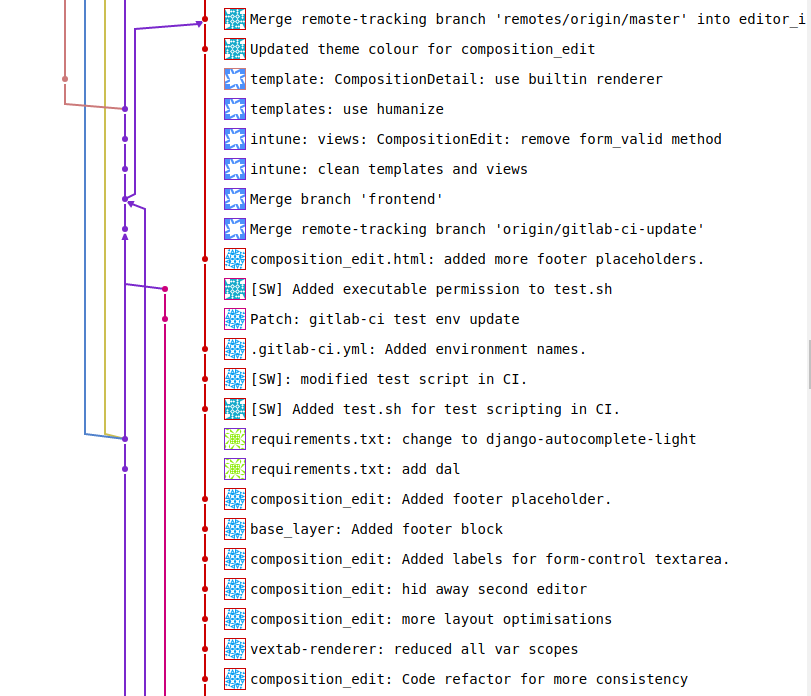
\includegraphics[width=\textwidth]{graph-mid}
        \caption{Commits in the middle of an iteration}
    \end{subfigure}
\end{figure}

\begin{figure}
    \centering
    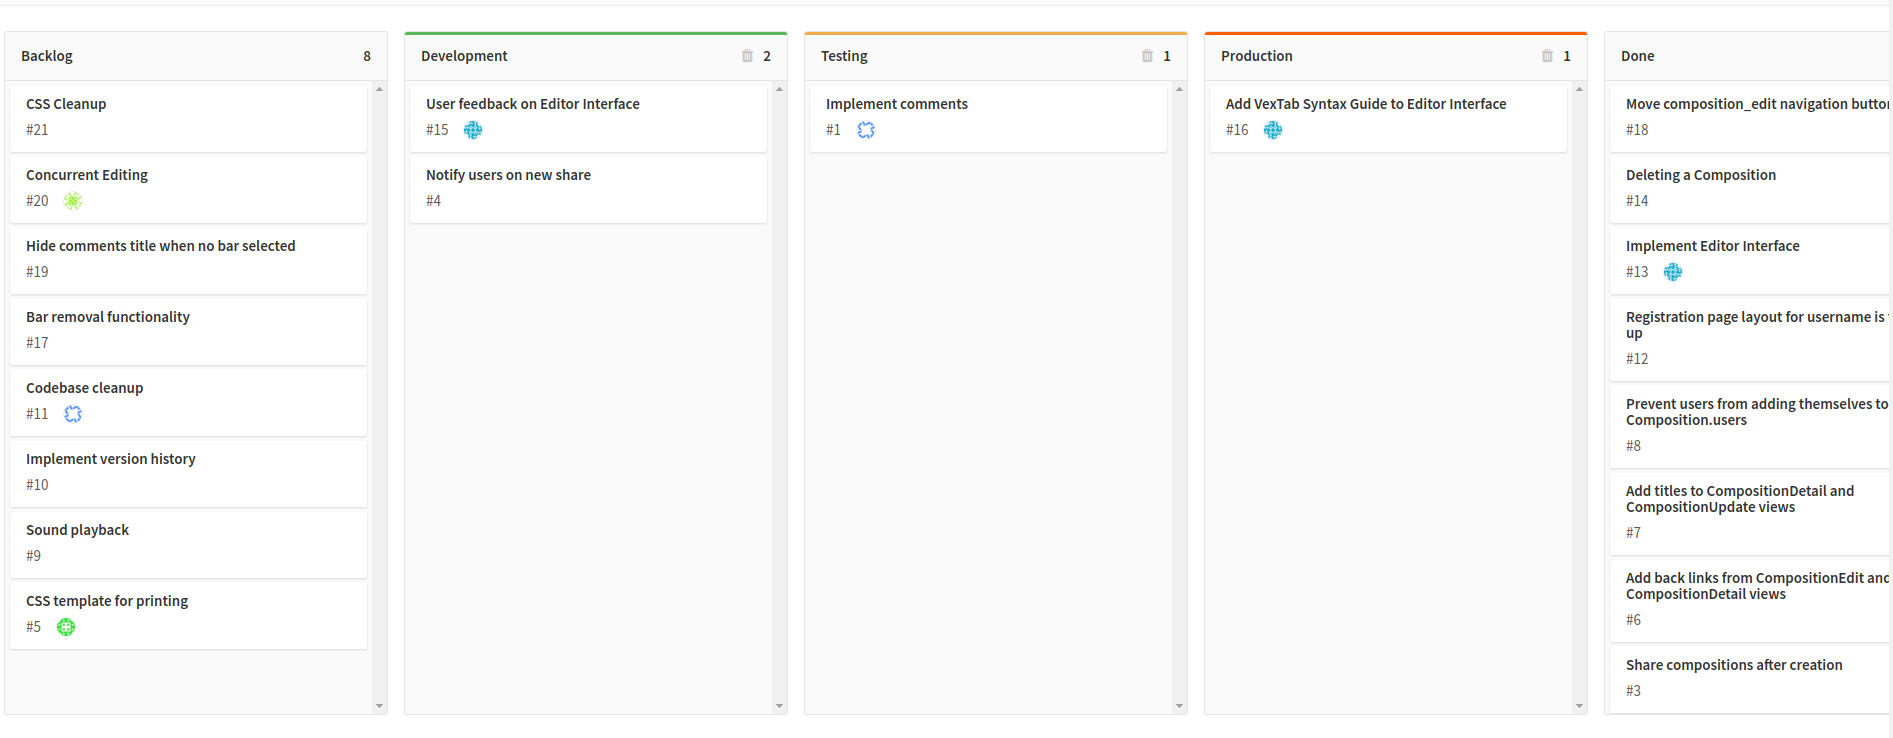
\includegraphics[width=0.65\textwidth]{issues-beg}
    \caption{Issue tracker at the beginning of an iteration}
\end{figure}

\begin{figure}
    \centering
    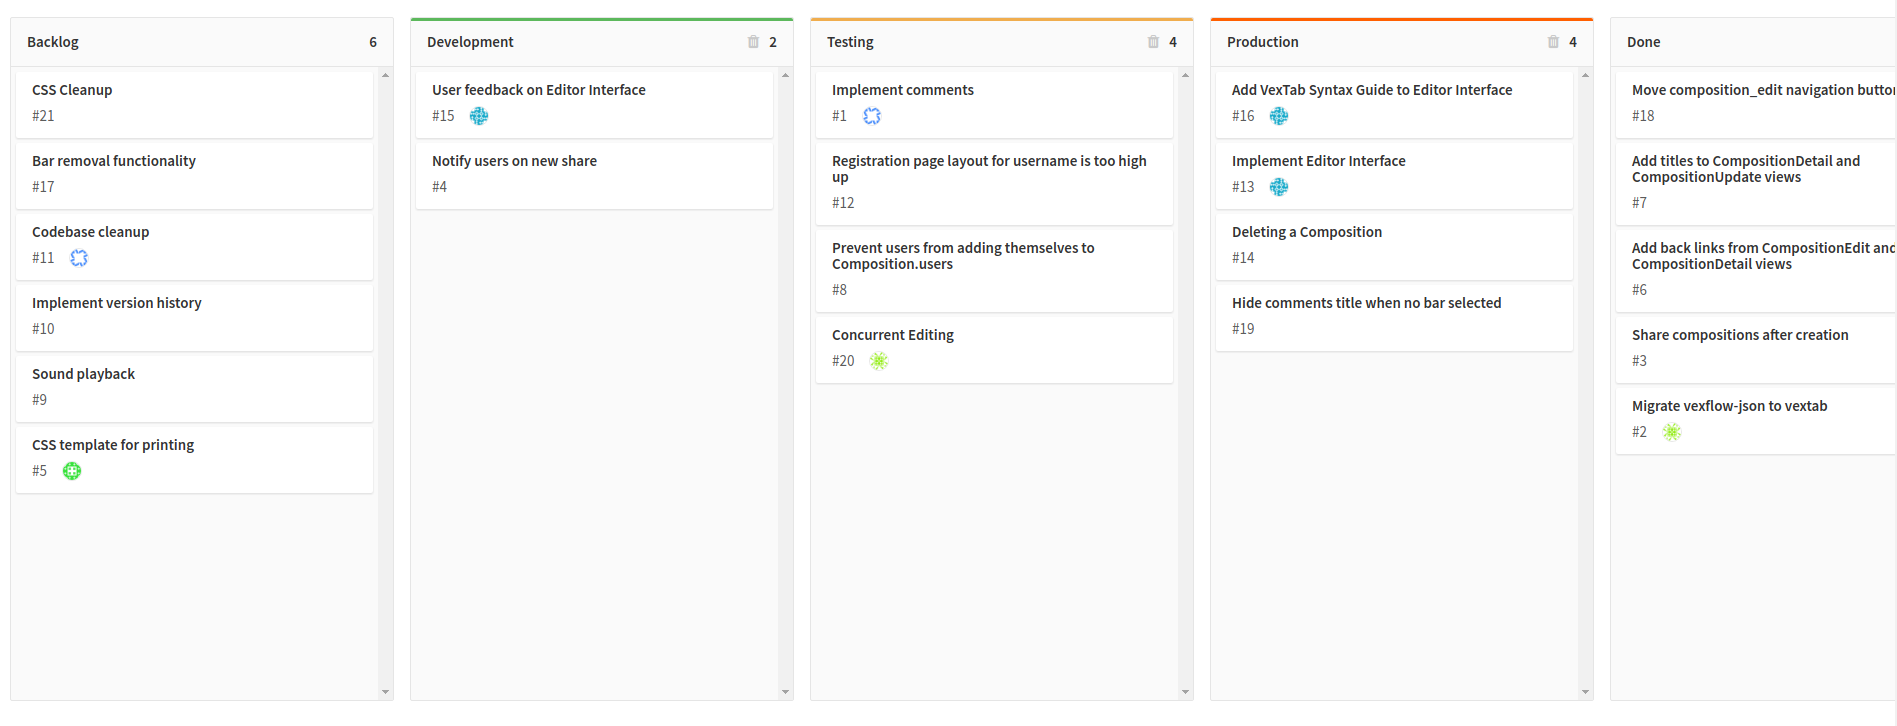
\includegraphics[width=0.65\textwidth]{issues-end}
    \caption{Issue tracker at the end of an iteration}
\end{figure}

At the end of an iteration/beginning of the next, we discuss what is needed to be done, and create branches accordingly. As work progresses, we merge branches to test features together and get feedback. Toward the end of the iteration, we consolidate our work, test, and deploy.

While the workflow provides structure, it is a little chaotic with one-week iterations, as deadlines cannot be too rigid.

\end{document}
